\documentclass[a4paper,12 pt]{report}
\usepackage{latexsym}
\usepackage[utf8]{inputenc}



%\usepackage[english]{babel}
\usepackage[italian]{babel}

\usepackage[protrusion=true,expansion=true]{microtype}	
\usepackage{amsmath,amsfonts,amsthm} % Math packages
\usepackage[pdftex]{graphicx}	
\usepackage{mathtools}

\usepackage{hyperref}
\usepackage[table,xcdraw]{xcolor}
\usepackage{setspace}
\usepackage{amssymb}
\usepackage{listings}
\usepackage{url}

\usepackage{xcolor}
\usepackage[T1]{fontenc}
\newcommand\myworries[1]{\textcolor{red}{#1}}

\usepackage{enumitem}
\usepackage{float}
\usepackage{hyperref}
\usepackage{tikz}
\usepackage{multirow}
\usepackage{todonotes}
\usepackage{placeins}

\usepackage{graphicx}  
\usepackage{array}
\usepackage{booktabs} 
\usepackage{pifont}
\newcommand{\xmark}{\ding{55}}
\newcommand{\cmark}{\ding{51}} 

\usepackage[square,numbers]{natbib}

%per pseudocodice
\usepackage{algorithm} 
\usepackage{algorithmic}
\floatname{algorithm}{Algoritmo}
\renewcommand{\thealgorithm}{\unskip}
\newlength\myindent
\setlength\myindent{2em}
\newcommand\bindent{%
	\begingroup
	\setlength{\itemindent}{\myindent}
	\addtolength{\algorithmicindent}{\myindent}
}
\newcommand\eindent{\endgroup}
\usepackage{listings}
% package italiano
%
% Opzionale
%
%\renewcommand{\contentsname}{Sommario}
%\renewcommand{\listfigurename}{List of Figures}
%\renewcommand{\listtablename}{List of Tables}
%\renewcommand{\bibname}{Bibliografia}
%\renewcommand{\indexname}{Indice}
%\renewcommand{\figurename}{Figura}
%\renewcommand{\tablename}{Tavola}
%\renewcommand{\partname}{Parte}
%\renewcommand{\chaptername}{Capitolo}
%\renewcommand{\appendixname}{Appendice}
%\renewcommand{\abstractname}{Abstract}
%\renewcommand{\footnotesize}{\scriptsize}
%\renewcommand{\today}{\ifcase\month\or
%  Gennaio\or Febbraio\or Marzo\or Aprile\or Maggio\or Giugno\or
%  Luglio\or Agosto\or Settembre\or Ottobre\or Novembre\or Dicembre\fi
%  \space\number\day, \number\year}

% package formato
\pagestyle{plain}
\setlength{\topmargin}{0.0in}
\setlength{\headheight}{0.1in}
\setlength{\headsep}{0.0in}
\setlength{\footskip}{0.8in}
\setlength{\textheight}{9.0in}
\setlength{\textwidth}{6.0in}
\setlength{\oddsidemargin}{0.2in}
\setlength{\evensidemargin}{0.2in}
\setlength{\parindent}{0.4 in}
\onehalfspacing


\def\cent{\centerline}
\def\vs{\vskip 10 pt plus 1 pt}
\def\bs{\bf}
\def\grad{\vec{\nabla}}
\def\gradx{\vec{\nabla}_x}
\def\epsilon{\varepsilon}



\newcommand{\cvd}{\begin{flushright}$\Box$\end{flushright}}
\newcommand{\tr}{{\rm Tr}\;}
\newcommand{\eq}{\begin{equation}}
\newcommand{\feq}{\end{equation}}
\theoremstyle{definition}
\newtheorem{definition}{Definition}[section]
 
\theoremstyle{remark}
\newtheorem*{remark}{Remark}

\definecolor{blu_dmi}{HTML}{002e62}


%%%%%%%%%%%%%%%%%%%%%%%%%%%%%%%%%
%%%%%%%%%%%%%%%%%%%%%%%%%%%%%%%%%
%%%%%%%%%%%%%%%%%%%%%%%%%%%%%%%%%
%%%%%%%%%%%%%%%%%%%%%%%%%%%%%%%%%



\begin{document}
    
\thispagestyle{empty} %suppress page number

	\noindent % just to prevent indentation narrowing the line width for this line
	
\includegraphics[width=0.15\textwidth]{img/logoUniPg}
	\begin{minipage}[b]{0.7\textwidth}
		\centering
		{\Large{\textsc{Universit{\`a} di Perugia}}}\\
		\vspace{0.4 em}
		{\large {Dipartimento di Matematica e Informatica}}
		\vspace{0.6 em}
	\end{minipage}%
	
\includegraphics[width=0.15\textwidth]{img/logoDMI}
	
	\vspace{8 em}

	\begin{center}
		

	
		{\Huge{Appunti Simulazione}}\\
		\vspace{2 em}
		{\large { Autore: Chiara Luchini}}\\
		\vspace{5 em}
		{\large {Basati su:}}\\
		{\large {- Slides del Prof. Sergio Tasso}}\\
		{\large {- Lezioni del Prof.Sergio Tasso}}\\

		
		\vspace{6 em}
		\vfill
		
	{\rule{380pt}{.4pt}}\\
		\vspace{1.2 em}
		\large{{Anno Accademico 2021/2022}}
		
		
		
		
	\end{center}

% ------------------------------------------------------------------
    \newpage
  	\tableofcontents
    \newpage
    %\lstlistoflistings
	\newpage
	\listoffigures
    \newpage
    \chapter{Sistemi e Modelli}
In questa Capitolo vengono introdotti i concetti e una classificazione dei sistemi e
dei modelli ed il procedimento di creazione ed uso di un modello al fine di valutare le
prestazioni del sistema rappresentato.

\section{Definizione di sistemi e modelli}
Un sistema è rappresentato come un insieme di componenti (elementi, entità) interdipendenti e che interagiscono per raggiungere un determinato obiettivo. Un sistema di elaborazione è composto da componenti software, hardware e firmware che permettono l'elaborazione delle informazioni eseguendo programmi di utente.\\
Nello studio di un sistema devono essere considerati vari fattori fra cui:
\begin{itemize}
    \item funzionalità e correttezza;
    \item affidabilità;
    \item costo e fattori economici;
    \item prestazioni.
\end{itemize}
Le fasi di sviluppo e progettazione di un sistema sono:
\begin{itemize}
    \item \textbf{fase di progettazione:} in questa fase si sceglie il progetto del sistema fra diverse configurazioni disponibili;
    \item \textbf{fase di dimensionamento e acquisizione:} comprende la scelta fra diversi sistemi o componenti disponibili;
    \item \textbf{fase di evoluzione della configurazione e del carico:} si considerano tutti gli aspetti e i problemi relativi alla modifica ed evoluzione di un sistema esistente.
\end{itemize}
Le metodologie per la valutazione delle prestazioni di sistemi possono essere suddivise in due categorie:
\begin{itemize}
    \item tecniche di misurazione;
    \item tecniche modellistiche.
\end{itemize}
Le prestazioni possono essere quantificate tramite  di merito o indici di prestazioni che ne descrivono l'efficienza.
\begin{figure}[H]
	\centering
    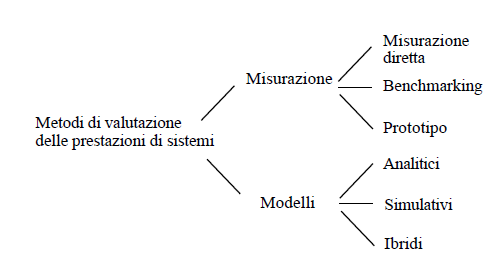
\includegraphics[width=15cm, keepaspectratio]{img/prestazioni.png}
	\caption{Metodi di valutazione delle prestazioni.}\label{fig:prestazioni}
\end{figure}
Come si può vedere in Figura \ref{fig:prestazioni} esistono diverse tecniche di misurazione:
\begin{itemize}
    \item \textbf{misurazione diretta}: il sistema vine misurato utilizzando il carico reale;
    \item \textbf{benchmark (carico artificiale)}: si ripete più volte il procedimento di misurazione e si effettuano misurazioni comparative fra diversi sistemi sotto le stesse condizioni di carico;
    \item \textbf{prototipazione}: se il sistema non è disponibile si può ricorrere alla costruzione di un prototipo su cui fare le misurazioni.
\end{itemize}


\paragraph{Definizione modello.}Un \textbf{modello} è una rappresentazione astratta del sistema che include solo gli aspetti rilevanti che servono per lo studio del sistema. Esso è definito da un certo livello di astrazione, cioè il sistema viene descritto con un certo livello di dettaglio riportando solo le componenti e le interazioni fra quest'ultimi necessari allo scopo prefissato.
\paragraph{Tecniche modellistiche.}
Si possono distinguere due tipologie di tecniche di modellazione:
\begin{itemize}
    \item \textbf{modello analitico}: variabili e parametri rappresentano le componenti e il carico del sistema, mentre le interazioni sono rappresentate tramite delle relazioni fra queste quantità;
    \item \textbf{modello di simulazione}: replica il comportamento dinamico di un sistema nel tempo rappresentando le componenti e le interazioni in termini di relazioni funzionali. La valutazione di quest'ultimo richiede l'esecuzione di un programma di simulazione o simulatore.
\end{itemize}

\paragraph{Vantaggi e svantaggi di un modello.}
I principali vantaggi nell'utilizzo di un modello per lo studio di un sistema sono:
\begin{enumerate}
    \item aumento e organizzazione delle conoscenze;
    \item analisi del sistema;
    \item modificabilità;
    \item diversi obbiettivi di studio.
\end{enumerate}
Invece gli svantaggi sono i seguenti:
\begin{enumerate}
    \item scelta del modello;
    \item uso errato del modello.
\end{enumerate}
 I modelli  che si basano su \textbf{processi stocastici} permettono di valutare la dinamica dei sistemi e in particolare le loro prestazioni e affidabilità. \\
 I \textbf{modelli a reti di code} permettono di rappresentare \textbf{sistemi di congestione}, i quali sono sistemi formati da un insieme limitato di risorse e in cui si osserva competizione per il loro utilizzo da parte di un insieme di utenti. Alcuni esempi di questi sistemi sono i sistemi di calcolo, di comunicazione. di traffico e di produzione. La valutazione delle prestazioni di un sistema di congestione include due differenti aspetti: dal punto di vista del sistema, si è interessati alla valutazione della utilizzazione delle risorse, mentre dal punto di vista dell’utente si valutano i tempi di attesa per l’uso delle risorse.
 
 \section{Classificazione di sistemi e di modelli}
 L'evoluzione nel tempo di un sistema è descritto dallo \textbf{stato} del sistema in ogni istante che ne rappresenta la condizione. Lo stato è espresso come \textbf{variabili di stato} che ne descrivono le entità e i loro attributi. Le attività delle componenti nel tempo e le interazioni fra queste sono descritte dalle \textbf{regole di trasformazione} fra stati. Il comportamento di un sistema nel tempo è rappresentato dalla \textbf{storia degli stati}. Le variabili di stato si distinguono in:
 \begin{itemize}
     \item \textbf{variabili endogene:} il loro cambiamento è dovuto soltanto ad attività interne al sistema. Il sistema si dice chiuso se il suo comportamento è determinato da queste variabili. 
     \item\textbf{ variabili esogene}: il loro cambiamento è influenzato dall'ambiente esterno al sistema. Il sistema si dice aperto se interagisce con l'ambiente esterno, utilizza anche variabili esogene. 
 \end{itemize}
 I sistemi possono essere suddivisi in \textbf{continui} e \textbf{discreti} a seconda del tipo di cambiamento dei valori delle variabili di stato, ad esempio se controlliamo la temperatura in un luogo la variabile che la rappresenta è continua poiché verifichiamo i cambiamenti nel tempo.\\
 Il modo in cui avvengono le trasformazioni fra stati determina se un sistema è \textbf{deterministico} o \textbf{stocastico}, nel primo caso le regole di trasformazione determinano il cambiamento del sistema in modo univoco mentre nel secondo si può passare da uno stato a un altro secondo diverse leggi/distribuzioni di probabilità. La natura del sistema dipende anche dalla visione dell'osservatore che è definita dagli obiettivi e dal metodo di studio. A loro volta anche i modelli possono essere distinti in queste categorie con la differenza che un modello associato un sistema non deve necessariamente corrispondergli, esempio un sistema deterministico definito da un modello stocastico. \\
 I modelli si distinguono in due principali categorie:
 \begin{itemize}
     \item modelli fisici;
     \item modelli simbolici: questi includono i modelli matematici e non.
 \end{itemize}
 
 
 
\section{Ciclo dei modelli}
Il procedimento di creazione di un modello è un processo iterativo di raffinamenti successivi, vengono fatte delle assunzioni ed ipotesi da verificare e valutare.
Il processo di creazione ed uso di un modello può essere schematizzato come segue:
\begin{enumerate}
    \item \textbf{Definizione degli obiettivi:} definizione e comprensione del sistema oggetto di studio e delle sue componenti. Si stabiliscono anche i criteri di valutazione delle soluzioni e si acquisiscono i dati dal sistema misurandone anche il carico.
    \item \textbf{Definizione del modello e formulazione delle assunzioni e ipotesi:} vengono identificate le componenti del modello così come le assunzioni ed ipotesi utilizzate.
    \item \textbf{Parametrizzazione:} sono identificate le variabili del modello da misurare e gli strumenti di misurazione.
    \item \textbf{Valutazione (soluzione) del modello e interpretazione dei risultati:} definito e parametrizzato il modello si sceglie il metodo di soluzione più appropriato.
    \item \textbf{Validazione del modello e valutazione dei risultati:} si valuta il modello nella descrizione del sistema se questo risulta non soddisfacente si itera ai passi 1, per ridefinire il sistema e gli obiettivi, o 2, per modificare la definizione del modello e delle ipotesi, o 3, per ri-parametrizzare le variabili.
    \item \textbf{Documentazione e analisi della sensitività:} riporta i risultati trovati compresi i dettagli relativi al modello e anche una descrizione del processo di definizione del modello.
\end{enumerate}

\begin{figure}[H]
	\centering
    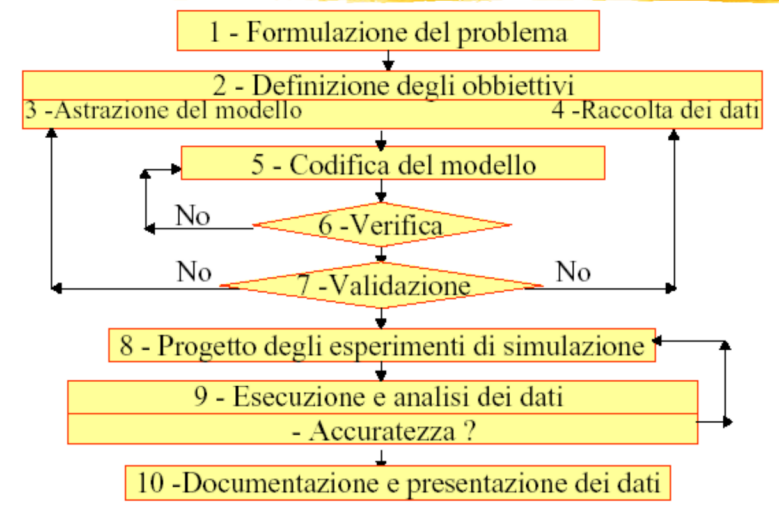
\includegraphics[width=15cm, keepaspectratio]{img/ciclo_modello.png}
	\caption{Ciclo di vita di un modello.}\label{fig:ciclo_modello}
\end{figure}

\section{Schemi di simulazione}
Sono delle strutture di modelli di simulazione che differiscono in base ai tre concetti di evento, attività e processo. Ne esistono quattro metodologie:
\begin{itemize}
    \item Interazione fra processi
    \item Scheduling di eventi
    \item Scansione di attività
    \item Metodo a Tre fasi
\end{itemize}

\subsection{Schemi di simulazione: processi}
Il flusso di esecuzione di un processo permette di simulare il comportamento di un oggetto (entità) attraverso il sistema. L'esecuzione del processo continua fintanto che non viene bloccato, sospeso o arriva un'altra entità. Nel caso in cui il flusso viene bloccato, si avanza nel tempo fino ad arrivare al punto di inizio dell'esecuzione della prossima attività.
\paragraph{Esempio: scheduling dei processi}
In un sistema di elaborazione ogni processo viene eseguito ciclicamente supponiamo che si utilizzi la disciplina FIFO per gestire la coda di processi, i passi eseguiti sono i seguenti:
\begin{enumerate}
    \item Esamina la coda, se vuota vai a 5
    \item Preleva un job dalla coda
    \item Esegui il servizio per il job
    \item Vai al passo 1
    \item Attendi l'arrivo del prossimo utente, quando arriva vai al passo 1
\end{enumerate}
Il punto 4 è un punto di sospensione o si riattivazione del processo, al contrario nel passo 5 il processo è in stato passivo fino a che non arriva un job. In generale nella simulazione fra processi esiste una routine che gestisce i cambiamenti di stato dei processi, essa controlla due code diverse:
\begin{itemize}
    \item \textbf{processi bloccati}: contiene gli oggetti sospesi
    \item \textbf{processi sospesi}: contiene gli oggetti passivi
\end{itemize}
La routine permette di riattivare un oggetto, il quale può essere:
\begin{itemize}
    \item \textbf{attivo:} esegue azioni
    \item \textbf{sospeso:} ha un tempo di riattivazione
    \item \textbf{passivo:} non è attivo e il tempo di riattivazione dipende da un altro oggetto
    \item \textbf{terminato:} ha terminato il suo lavoro
\end{itemize}

\subsection{Schemi di simulazione: eventi}
Nella simulazione per scheduling di eventi si avanza il tempo simulato al tempo del prossimo evento che coincide spesso con il termine di un'attività o l'inizio. In questo caso gestiamo una lista ordinata di eventi e scheduler di eventi. Lo scheduler di eventi gestisce il tempo simulato mantenendo una lista ordinata di eventi futuri:
\begin{itemize}
    \item \textbf{event-driven}: clock= tempo del prossimo evento in lista
    \item \textbf{unit-time:} $clock= clock + \Delta$
\end{itemize}
Inoltre esso gestisce anche la struttura dati che contiene tutti gli eventi e anche la routine evento.
Quest'ultima permette di aggiornare sia la lista di variabili di stato che la lista di eventi, essa può essere di:
\begin{itemize}
    \item \textbf{inizializzazione}:chiamata per prima e definisce le variabili di stato ed altro;
    \item \textbf{gestione degli eventi};
    \item \textbf{ trace}: serve per notificare eventi o stime a run-time;
\end{itemize}


\subsection{Schemi di simulazione: attività}
La simulazione avviene scansionando le attività ovvero descrivendone le componenti del modello. Se è applicato il meccanismo di avanzamento per intervalli fissi $\Delta$, ad ogni avanzamento vengono esaminate tutte le attività per stabilire le condizioni di inizio e di fine. Le procedure aggiornano lo stato della singola attività. Si può anche applicare un meccanismo di avanzamento del tempo distribuito nelle procedure delle attività simile all'avanzamento per eventi.

\subsection{Schemi di simulazione: "tre fasi"}
Nella simulazione a "tre fasi" si ha un avanzamento del tempo per intervalli fissi, le varie fasi che la compongono sono:
\begin{itemize}
    \item  fase 1: avanzamento del tempo simulato;
    \item fase 2: rilascio risorse mantenute dalle attività che risultano terminate dopo l'avanzamento;
    \item fase 3: esecuzione delle attività per la quali siano ora disponibili le risorse.
\end{itemize}


 	\newpage
    \chapter{Fondamenti di Calcolo delle Probabilità e Statistica}
In questo Capitolo verranno riportate alcune nozioni base di Probabilità e Statistica applicabili nel campo della simulazione informatica, indispensabili per la costruzione e l’uso di
modelli di simulazione stocastica.

\section{Variabili stocastiche}
Un modello di simulazione è un modello intrinsecamente stocastico. Infatti i valori usati per le variabili di ingresso, di stato iniziale e i parametri sono decisi a partire dal sistema reale attraverso delle misurazioni fisiche, ogni valore appartiene a una distribuzione di probabilità. Perciò abbiamo bisogno di ripassare alcune nozioni base della probabilità in modo da comprendere i valori estratti da queste distribuzioni.\\

Una variabile stocastica o aleatoria $x_i$ rappresenta l'uscita di un'attività casuale. Essa può assumere n differenti valori dato $i ={1,2,...,n}$, ciascuno con una determinata probabilità $p_i(x) = p_1,p_2,...,p_n$.\label{fun_prob} L'insieme di tutte le probabilità è detto \textbf{funzione discreta di probabilità}. Da ricordare che la somma di tutte le singole probabilità da come risultato 1, ovvero:
\[ \sum_{i=1}^{n} p_i(x) = 1\]

\noindent Esse possono essere definite anche nel seguente modo.\\
Uno spazio di probabilità è una tripla $(\Omega, \mathcal{F}, P)$ dove:
\begin{itemize}
    \item $\Omega$ è lo spazio campione, il quale è un insieme di elementi (spesso l'insieme dei possibili esiti);
    \item $\mathcal{F}$ è lo spazio degli eventi, il quale è una famiglia di sottoinsiemi di $\Omega$ che ha le seguenti proprietà:
    \begin{enumerate}
        \item  $\Omega \in \mathcal{F} $,
        \item $A \in \mathcal{F} \Rightarrow \Omega \setminus A \in \mathcal{F}$,
        \item $A,B \in \mathcal{F} \Rightarrow A \cup B \in \mathcal{F} $.
    \end{enumerate}
    \item $P: \mathcal{F} \rightarrow [0,1]$ è la funzione di probabilità (definita come $p(x)$ in \ref{fun_prob}), la quale è una funzione reale con la seguenti proprietà:
    \begin{enumerate}
        \item $P(A) \geq  0 ,\forall \in \mathcal{F}$,
        \item $P(\Omega) = 1$,
        \item $(A, B \in \mathcal{F}) \wedge(A \cap B=\emptyset) \Longrightarrow P(A \cup B)=P(A)+P(B)$.
    \end{enumerate}
\end{itemize}

Dato uno spazio di probabilità, una variabile casuale è una funzione $ X : \Omega \rightarrow \Re$ che ha la seguente proprietà, per ogni reale $r$, $\{\omega \in \Omega: X(\omega) \leq r\} \in \mathcal{F}$. La funzione $F_X(x) = P(X \leq x = P( \{\omega \in \Omega: X(\omega) \leq r\})$, definita sull'insieme dei reali, è detta \textbf{funzione di distribuzione}.
Le variabili stocastiche o casuali vengono utilizzate poiché nei sistemi da simulare spesso si presentano degli eventi non facilmente prevedibili a priori, come ad esempio l'arrivo di clienti ad uno sportello o la quantità di pioggia in una determinata stagione. Perciò tali fenomeni vengono rappresentati tramite queste variabili dalle quali estrarne poi la distribuzione di probabilità.

\paragraph{Esempio} Si consideri il numero di pazienti che si presentano ad un
ambulatorio tra le 9 e le 10 di mattina, e poniamo $\Omega = {0, 1, 2, . . .}$, $\mathcal{F}= 2^\Omega$ ,
e $X(\omega) = \omega$ (la funzione identità). La funzione X così definita è una variabile
casuale, infatti, per ogni reale $r$ è
\[ \{\omega \in \Omega: X(\omega) \leq r\} = \{0,...,\left \lfloor r \right \rfloor\} \in \mathcal{F}\]


\subsection{Funzione densità di probabilità}
La \textbf{funzione densità di probabilità $f(x)$} si utilizza per definire la probabilità di una variabile di assumere uno specifico valore tra infiniti valori , la quale è praticamente nulla, a causa del processo osservato che è continuo. Detto ciò essa si può definire come la probabilità che $ x_1 \leq x \leq x_2$, ovvero che il valore di x sia compreso in intervallo $[x_1, x_2]$, data da:
\begin{align*}
     & p(x_1 \leq x \leq x_2) = \int_{x_1}^{x_2}f(x) d(x)= \\
     &  \int_{-\infty }^{+ \infty} f(x) dx = 1
\end{align*}
   
\subsection{Funzione cumulativa di distribuzione}
La \textbf{funzione cumulativa di distribuzione $F(x)$} definisce la probabilità che un certo valore sia minore o uguale a x, la quale si può descrivere come:
\[ F(x) = \int_{- \infty}^{X}f(x) d(x) \]
Da cui risulta che $0 \leq F(x) \leq 1$ e $p( x_1 \leq x \leq x_2) = F(x_2) - F(x_1)$.

\subsection{Media}
Per una variabile discreta \footnote{Una variabile casuale è detta \textbf{discreta} se l'insieme di valori che può assumere è numerabile.} si definisce il \textbf{valore atteso} o \textbf{media $E(x)$ oppure $\mu_x$} come:
\[ E(x) =  \sum_{i=1}^{n} x_i p_i(x)\]
Si definisce media di una funzione $y=g(x)$:
\[ E(g(x)) = \sum_{i=1}^{n} g(x_i) p_i(x)\]
Per una variabile continua si ha che la media è pari a:
\[ E(x) = \int_{-\infty}^{+ \infty} xf(x)dx = \lambda_1 = \lambda\]
e per una funzione continua y:
\[ E(x) = \int_{-\infty}^{+ \infty} g(x)f(x)dx = \int_{-\infty}^{+ \infty} g(x)dF(x)\]

Altro...

\subsection{Varianza}
Si definisce \textbf{varianza} di x e si indica con $\sigma^2(x)$, è la media degli scarti quadratici rispetto alla media $\mu_x$ e rappresenta una misura di dispersione di x. La sua radice quadrata, $\sigma_x$ è detta \textbf{deviazione standard}. La varianza è definita come 
\[ \sigma^2(x) = E(x-\lambda)^2 = \int_{-\infty}^{+\infty}(x-\lambda)^2 f(x)dx  \]
Da cui si ricava facilmente
\[\sigma^2(x) = E(x^2) - E^2(x)\]
Se x è una \textbf{variabile discreta} si ha
\[ \sigma^2(x) = \sum_{i=1}^{n}(x_i -E(x))^2 \cdot p_i(x)\]
La deviazione standard viene definita come
\[ \sigma(x) = \sqrt{\sigma^2(x)}\]
\subsubsection{Teorema di Beniaymé-Chebychev}
Il Teorema di Beniaymé-Chebychev lega la deviazione standard di x alla probabilità di deviazione dei singoli valori di x della media:
\[ p(\left | x- \lambda \right | \geq k\sigma) \leq \frac{1}{k^2}   \]
 Ovvero, qualunque sia la forma di $f(x)$, la probabilità al di fuori di $\pm k \sigma$ è limitata, $\leq \frac{1}{k^2}$.
 
 \subsection{Funzione di probabilità di due variabili aleatorie} \label{subsec:prob_congiunta}
 In modo analogo al precedente si definisce la funzione di distribuzione $F(X,Y)$ di due variabili aleatorie x e y
 \[ F(X,Y) = p(x \leq X, y \leq Y)\]
 che indica la probabilità che $x \leq X$ ,valore prefissato, e $y \leq Y$. La suddetta funzione è detta anche \textbf{funzione di probabilità congiunta} e scritta $F(x,y)$.
 Da essa possiamo ottenere la definizione di \textbf{densità congiunta di probabilità}. Nel caso di variabili discrete data l'esistenza di un insieme numerabile di punti 
 \[ (X_1, Y_1), (X_1,Y_2),...,(X_2,Y_2),...,(X_i,Y_j)\]
 con associati numeri positivi 
 \[\ p_{11},p_{12},...,p_{21},p_{22},...,p_{ij}\]
\noindent i quali soddisfano la relazione $F(X_h, Y_k) = \sum_{i}^{}\sum_{j}^{}p_{ij}$ con $\sum_{i}^{}\sum_{j}^{}p_{ij}=1$ sommata per tutti gli i e j per i quali $X_i \leq X_h$ e $Y_j \leq Y_k$.
Allora si può definire $p = (x=X_i, y=Y_j) = p_{ij}$ per tutti gli i e j per i quali esistono dei valori delle variabili x e y, assumendo $p_{ij} = 0$ altrove. Quindi la \textbf{funzione discreta di probabilità congiunta} è $f(x_i, y_j) = p_{ij}$ con distribuzione cumulativa $F(x_i,y_j)$.\\
Se invece la funzione F(x,y) è continua si definisce la \textbf{densità congiunta}
\[f(x,y) = \dfrac{\lambda}{\lambda x} \dfrac{\lambda}{\lambda y} F(x,y) \] e quindi
\[F(x,y) = \int_{-\infty}^{y}\int_{-\infty}^{x} f(x,y) dxdy\]
\[ p(a \leq x\leq b , c \leq y \leq d) = \int_{c}^{d}\int_{a}^{b} f(x,y) dxdy \]
\[ p( X \leq x \leq X + dX , Y \leq y \leq Y +dY) = F(X,Y) dXdY\]

\subsection{Distribuzione marginale}
Si vuole determinare la probabilità g(x) e h(y) di una variabile x o y, data la densità congiunta f(x,y) di due. In poche parole la \textbf{distribuzione marginale} di un sottoinsieme di una collezione di variabili casuali è la distribuzione di probabilità delle variabili contenute nel sottoinsieme. Ciò si interpreta dicendo che si vuole la $p(x \leq X, $con y qualunque$)$ simboleggiata con $F(x, \infty)$ o $F(\infty,y)$.
Nel caso discreto si ha 
\[F(x_h, \infty) = \sum_{i}^{}\sum_{j}^{}p_{ij}\] 
Nel caso continuo si ha invece 
\[ F(x,\infty)=\sum_{-\infty}^{X} \sum_{-\infty}^{\infty} f(x,y) dxdy= \int_{-\infty}^{X} g(x) dx \]
Da cui si ha 
\[g(x) = \int_{-\infty}^{\infty}f(x,y) dy \]
\[h(y) = \int_{-\infty}^{\infty}f(x,y) dx \]

dove g(x) e h(y) sono dette \textbf{distribuzioni marginali} di x e y.

\subsection{Indipendenza}
Due variabili aleatorie x e y sono dette \textbf{indipendenti} se , detta f(x,y) la loro densità congiunta e g(x) e h(y) le relative distribuzioni marginali si ha:
\[ f(x,y) = g(x) \cdot h(y)\]
La condizione necessaria e sufficiente alla validità della formula sopra è che f(x,y) può essere fattorizzata nel prodotto di due funzioni, ovvero:
\[f(x,y) = r(x) \cdot s(y)\]

\subsection{Variabili completamente dipendenti e variabili stocasticamente correlate}
Per coppie di variabili dipendenti si ha che f(x,y)=g(x)=h(y), ovvero la probabilità f(x,y) è uguale a 0 solo per coppie x,y dove y è una funzione ad un solo valore di x e viceversa.
In tutti i casi in cui f(x,y) non è né il prodotto $g(x) \cdot h(y)$ né tale che g(x)=h(y)=f(x,y) le variabili x e y si dicono stocasticamente correlate.
Il coefficiente di correlazione misura il grado di correlazione il quale è pari a:
\begin{itemize}
    \item 0 se e solo se $f(x,y) = g(x) \cdot h(y)$
    \item $|1|$ se e solo se $f(x,y)=g(x)=h(y)$
    \item $0\leq |x| \leq 1$ in tutti gli altri casi.
\end{itemize}

\subsection{Probabilità condizionali}
La \textbf{probabilità condizionale} identifica la probabilità che una variabile x assuma il valore $x_i$, assunto che y assuma il valore $y_j$ si scrive:
\[p(x=x_i|y=y_j) = \dfrac{p(x=x_i,y=y_j)}{p(y=y_j}= \dfrac{f(x_i,y_j)}{h(y_j)}= g(x_i|y_j)\]
Si possono scrivere le funzioni densità condizionali di probabilità di x dato y e di y dato x:

 \begin{align*}
     g(x|y) =\dfrac{f(x,y)}{h(y)} \\
     h(y|x) = \dfrac{f(x,y)}{g(x)}
 \end{align*}
 
 Nel caso di variabili indipendenti di ha:
 \begin{align*}
     g(x|y) =g(x) \\
     h(y|x) = h(y)
 \end{align*}
 \subsection{Covarianza}
 La covarianza è una misura della relazione tra due variabili x e y, essa viene definita come di seguito:
 \[cov(x,y) = E(xy) - E(x)E(y)\]
 Dalla definizione risulta che:
\begin{itemize}
    \item cov(x,y)>0 se, nella funzione f(x,y) grandi valori di x sono associati a grandi valori di y e viceversa;
    \item cov(x,y)<0 se piccoli valori di x sono associati a grandi valori di y e viceversa;
    \item cov(x,y)=0 se, quando x è grande, alcuni valori di y sono grandi e alcuni piccoli.
\end{itemize}

\subsection{Coefficiente di correlazione}
Il \textbf{coefficiente di correlazione} p(x,y) tra due variabili si definisce come la misura standardizzata della covarianza e si scrive come:
\[p(x,y) = \dfrac{cov(x,y)}{\sigma(x) \sigma(y)}\]
Esso misura il grado di dipendenza lineare tra x e y. Il suo valore è compreso tra (-1,1), raggiungendo $\pm 1$ quando esiste una dipendenza perfettamente lineare tra x e y. Al contrario se x e y sono indipendenti allora si ha p=0, ma il contrario non è necessariamente vero. Questo vuol dire che se due variabili hanno p=0 sono dette \textbf{non correlate}, ma non è detto che siano indipendenti. Perciò l'uso di p come misura dell'indipendenza deve essere limitato a quei problemi che hanno una possibile dipendenza lineare.




\section{Generazione di numeri casuali}

\subsection{Metodo congruente lineare}
Il \textbf{metodo congruente lineare} serve per generare sequenze di interi compresi tra 0 e m da utilizzare per la generazione di distribuzioni uniformi, gli obiettivi da soddisfare sono:
\begin{enumerate}
    \item massimo periodo;
    \item granularità fine;
    \item efficienza di calcolo.
\end{enumerate}
Questo metodo usa la seguente funzione:
\[X_{i+1}=(aX_i + c) \text{mod m}\]
se c=0 il metodo di chiama \textbf{congruente moltiplicativo}.
La scelta dei parametri a= moltiplicatore e c= incremento è critica nel determinare il periodo e le doti di casualità. La funzione \verb|rand()| implementa il metodo congruente moltiplicativo con parametri $m= 2^31 -1 $ e $a=75$.

\subsection{Test del Chi-quadro $X^2$}
Per verificare le doti di casualità di una sequenza occorre sottoporla ad una serie di test:
\begin{itemize}
    \item Test del $X^2$
    \item Test seriale
    \item Test del gap
\end{itemize}
L'obiettivo di questi test è di verificare l'uniformità della distribuzione generata e la mancanza di correlazione tra numeri che si trovano ad una certa distanza k nella sequenza.
Per verificare l'uniformità si calcola:
\[V= \sum_{s=1}^{k}\dfrac{(Y_s - np_s)^2}{np_s}\]
Poi si confronta il valore ottenuto con la tabella dei percentili.
Il test del $X^2$ funziona nel seguente modo:
\begin{itemize}
    \item si dividono i possibili valori in k categorie;
    \item si genera un campione di n numeri e si contano le occorrenze di valori in ciascuna categoria $Y_s$;
    \item si calcola il valore atteso di valori in ciascuna categoria con la formula $p_s \cdot n$ dove $p_s$ è la probabilità di estrarre un valore nella categoria s;
    \item infine si calcola la sommatoria $V= \sum_{s=1}^{k}\dfrac{(Y_s - np_s)^2}{np_s}$.
\end{itemize}

\begin{figure}[H]
	\centering
    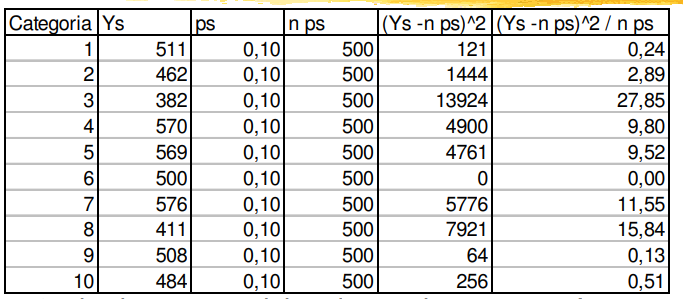
\includegraphics[width=15cm, keepaspectratio]{img/test_chi_quadro.png}
	\caption{Test del Chi-quadro.}\label{fig:chi_quadro}
\end{figure}

\subsection{Test per la verifica delle proprietà di casualità}
I valori $m= 2^31-1$, a=1 e c=1 garantiscono il periodo massimo e l'uniformità di distribuzione dei risultati ma non garantiscono l'assenza di correlazione fra i valori, per rilevare questo problema il test del $X^2$ può essere applicato a coppie di valori estratti dalla sequenza. Nell'esempio di prima si potrebbe dividere il range di valori in 5 sotto-range e formare 25 categorie corrispondenti a tutte le possibili coppie di sotto-range e la $p_s$ si calcola come prodotto delle probabilità di generare un valore in ciascuno di essi. Altri test sono quello del \textbf{gap} ovvero si calcola la lunghezza di sequenze i cui valori sono compresi tra $\alpha$ e $\beta$ e si confronta la loro distribuzione con quella teorica usando il chi-quadro.

\section{Generazione di distribuzioni qualsiasi}
Per la generazione di diverse distribuzioni si utilizzano i seguenti metodi:
\begin{itemize}
    \item\textbf{ Metodo della trasformazione inversa}
    \item \textbf{Metodo del rifiuto}
    \item \textbf{Metodo della composizione}
\end{itemize}

\subsection{Metodo della trasformazione inversa}
\begin{figure}[H]
	\centering
    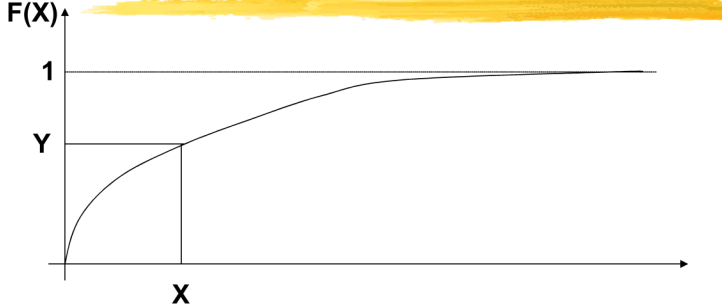
\includegraphics[width=15cm, keepaspectratio]{img/trasformazione_inversa.png}
	\caption{Trasformazione inversa.}\label{fig:trasformazione_inversa}
\end{figure}
Un esempio di applicazione del metodo è la generazione di variabili
casuali distribuite secondo una esponenziale negativa:
\begin{align*}
    & F(x) = 1 - e^{-\mu x} \\
    & 1-y = e^{- \mu x} \\
    & ln(1-y) = ln(e^{-\mu x}) = -\mu x\\
    & x = \dfrac{- ln(1-y)}{\mu}\\ 
\end{align*}
Se y è distribuita come U(0,1), anche Z = 1-Y ha la stessa distribuzione: quindi si può generare una sequenza distribuita secondo una esponenziale negativa semplicemente generando una sequenza con distribuzione U(0,1), applicando la funzione logaritmo naturale, cambiando di segno e dividendo per µ i numeri di tale sequenza.

\subsection{Metodo del rifiuto}
Quando non è facilmente ricavabile l'inversa della cumulativa si utilizzano altri metodi come il metodo del rifiuto.
\begin{figure}[H]
	\centering
    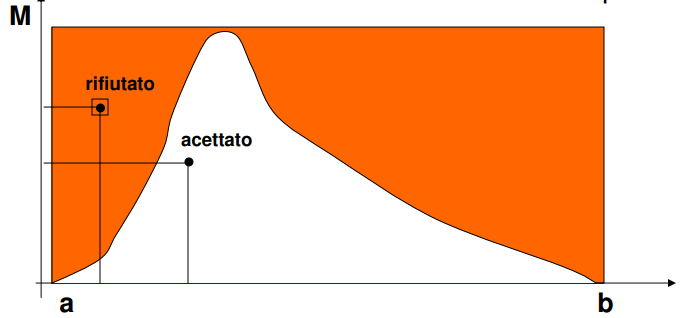
\includegraphics[width=15cm, keepaspectratio]{img/metodo_rifiuto.png}
	\caption{Metodo del rifiuto.}\label{fig:metodo_rifiuto}
\end{figure}
Si genera un valore y distribuito come U(0,M) e un x uniformemente distribuito tra a e b, se $y \leq f(x)$ allora si accetta x come valore generato della distribuzione, sennò si ripete con altri due valori di x e y.

\subsection{Metodo della composizione}
Questa distribuzione può essere vista come risultato della composizione di 4 uniformi: $U(a_1,a_2), U(a_2,a_3), U(a_3,a_4), U(a_4,a_5)$.
\begin{figure}[H]
	\centering
    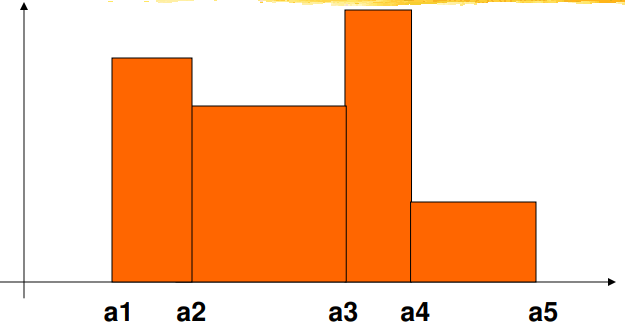
\includegraphics[width=15cm, keepaspectratio]{img/metodo_composizione.png}
	\caption{Metodo della composizione.}\label{fig:metodo_composizione}
\end{figure}
Siano $p_1, p_2, p_3$ e $p_4$ le aree dei quattro rettangoli: per generare un valore tratto da questa distribuzione scegliamo un rettangolo utilizzando le $p_i$, poi generiamo un numero uniformemente distribuito in $U(a_i, a_{i+1})$.

\section{Distribuzioni}
    \newpage
    \chapter{Processi stocastici}
I processi stocastici costituiscono una classe di modelli di sistemi che permette lo
studio e l’analisi dei sistemi. In questo Capitolo verranno riportate alcune definizioni e classificazioni dei suddetti processi, soffermando l'attenzione sui processi Markoviani.

\section{Processi stocastici}
Un \textbf{processo stocastico} è definito come una famiglia di variabili casuali $X = \{X(t) | t \in T\}$ definite in uno \textbf{spazio di probabilità} $\Omega$ ed indicate dal parametro \textbf{t}, dove t varia in un insieme T e indica il tempo. Ogni variabile casuale X(t) assume valori, detti \textbf{stati}, in un insieme E detto \textbf{spazio degli stati} del processo stocastico. Essendo che ogni variabile è definita come una funzione su uno spazio campione S, allora il processo stocastico è visto come un insieme di funzioni $\{ X(t,s) | t\in T, s \in S\}$.\\
I processi stocastici possono essere classificati in base alle seguenti caratteristiche:
\begin{itemize}
    \item spazio degli stati E
    \item indice tempo
    \item tipo di dipendenza stocastica fra le variabili casuali
\end{itemize}

\subsection{Spazio degli stati E}
Lo spazio degli stati può essere \textbf{discreto} o \textbf{continuo}. Nel primo caso il processo è detto anche catena e lo spazio E è indicato come l'insieme di interi non negativi. Nel secondo l'insieme dei valori assunti non è finito o numerabile perciò il processo è a spazio continuo.
\subsection{Indice tempo}
L'indice tempo è a sua volta \textbf{discreto} o \textbf{continuo}. Un processo a tempo discreto è anche detto sequenza stocastica ed è denotato come $\{X_n | n \in T \}$ dove T è finito o numerabile. Al contrario, se i cambiamenti avvengono in un qualsiasi istante di un tempo infinito allora si ha un processo a tempo continuo e si denota come $\{ X(t) | t\in T\}$.

\subsection{Dipendenza stocastica fra variabili}
La \textbf{dipendenza stocastica} fra variabili casuali X(t) per diversi valori di t è identificata dalla funzione di distribuzione di probabilità congiunta per le variabili $X= [X(t_1),X(t_2),...,X(t_n)]$, vedi \ref{subsec:prob_congiunta}, denotata come:
\[F_X(x;t) = Prob\{ X(t_1) \leq x_1; X(t_2) \leq x_2; ... ; X(t_n) \leq x_n \}\]
al variare di n e di $x= [x_1,x_2,...,x_n]$ e  $t= [t_1,t_2,...,t_n]$ con $x_i \in E$, $t_i \in T$ $1 \leq i \leq n$, $ n \geq 1$ e $t_1 \leq t_2 \leq ... \leq t_n$.

\subsubsection{Classificazione in base alla dipendenza stocastica}
Come accennato in precedenza è possibile classificare i processi in base alla dipendenza stocastica. \\
Un processo si dice \textbf{stazionario} in senso stretto se la funzione distribuzione $F_X (x;t)$ è invariante rispetto allo spostamento sull'asse del tempo T ovvero se per ogni $\tau$ costante
\[F_X (x; t+\tau) = F_X(x;t)\]
dove $t + \tau = [t_1+ \tau,t_2+\tau,...,t_n+\tau]$ e per ogni x,t e n.\\
Un processo stocastico è \textbf{indipendente}  se la funzione di distribuzione congiunta è
fattorizzabile nelle singole funzioni di distribuzione marginali:
\[ F_X(x;t)= \prod_{i=1}^{n} F_{X_{i}}(x_i;t_i) = \prod_{i=1}^{n} Prob\{ X(t_i) \leq x_i\}\]
Un processo stocastico è di\textbf{ rinnovamento} se le variabili casuali $X_1,X_2,...$ sono indipendenti, identicamente distribuite e a valori non negativi.

\subsection{Processi di Markov}
Un processo stocastico a tempo discreto $\{X_n |n \in T \}$ è di Markov se la probabilità di stato al tempo n+1 dipende soltanto dallo stato al tempo attuale,n, e non dalla storia precedente, ovvero se per ogni $n >0$ e per ogni valore degli stati $j,i_0,i_1,i_2,..., i_n \in E$ si ha:
\[Prob\{X_{n+1} = j | X_0 = i_0; X_1=i_1;...;X_n = i_n\} = Prob \{ X_{n+1} = j |X_n =i_n\}\]

Un processo stocastico a tempo continuo $\{X_n |n \in T \}$ è di Markov se per ogni sequenza di valori $t_0 \leq t_1\leq... \leq t_n< t$ la distribuzione di probabilità di X(t) condizionata a $X(t_0),X(t_1),..., X(t_n)$ dipende soltanto dallo stato $X(t_n)$, per ogni $n >0$ e per ogni valore degli stati $j,i_0,i_1,i_2,..., i_n \in E$ si ha:
\[Prob\{X(t) = j | X(t) = i_0; X(t_1)=i_1;...;X(t_n) = i_n\} = Prob \{ X(t) = j |X(t_n) =i_n\}\]

Per un processo di Markov a tempo discreto il tempo di permanenza in uno stato è un v.c. \textbf{geometrica} mentre per un processo di Markov a tempo continuo è un v.c. \textbf{esponenziale}. Questo vincolo deriva
dalla proprietà di assenza di memoria indotta sulla v.c. dal processo Markoviano. Come è noto le uniche distribuzioni che godono della proprietà di assenza di memoria sono, rispettivamente, la geometrica fra le distribuzioni discrete e l’esponenziale fra le continue. Se si assume che la distribuzione di probabilità non sia geometrica o esponenziale allora si ha un processo stocastico di semi-Markov, in questo caso le transizioni di tempo vanno ad istanti di tempo presi arbitrariamente. \\
Un p.s. di Markov a spazio discreto E è anche detta \textbf{catena di Markov}.
Una catena di Markov è di \textbf{nascita-morte} (birth-death) se le uniche transizioni possibili che il processo può effettuare sono soltanto fra stati vicini. Nel caso di tempo discreto, se lo stato $X_n=i$ allora lo stato al tempo successivo può soltanto essere $X_{n+1}\in{i-1, i, i+1}$. \\
Se lo spazio degli stati E è a tempo discreto allora $\{X_n | n \in N\}$ è una catena di Markov a tempo discreto, $X_n = j$ indica che il processo si trova nello stato j al tempo n, $n \in N$, $j \in E$. Nella formula della probabilità condizionata al membro destro:
\[Prob\{X_{n+1} = j | X_n = i\}\]

è detta probabilità di transizione al tempo n dallo stato i allo stato $j,i,j\in E, n \geq 0$.
Una catena di Markov si dice omogenea se le probabilità di transizione sono indipendenti dal tempo n. La probabilità di transizione dallo stato i allo stato j è definita come:
\[ p_{ij} = Prob\{X_{n+1} = j | X_n = i\}\]
$\forall i,j \in E, \forall n \geq 0$. \\
Una catena di Markov può essere analizzata sia in un tempo finito (\textbf{analisi transiente}, non importante per esame) sia a lungo termine (\textbf{analisi stazionaria}).

\subsection{Analisi stazionaria}
La descrizione del processo stocastico in condizioni asintotiche, per il tempo n che tende ad infinito, si esprime in termini di distribuzione di probabilità di stato. Sia $ \pi_j = \lim_{n \to \infty} \pi_j(n) = Prob\{X=j\}$ la probabilità di osservare lo stato j in condizioni di equilibrio, $\forall j \in E$. In forma compatta indichiamo con $\pi =[\pi_0, \pi_1. \pi_2,...,\pi_n]$ il vettore delle probabilità stazionarie di stato.

\subsubsection{Classificazione degli stati}
\begin{figure}[H]
	\centering
    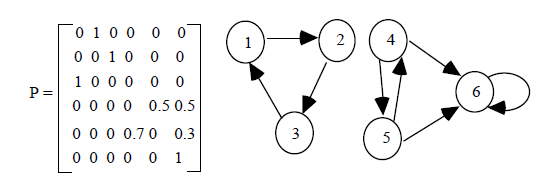
\includegraphics[width=15cm, keepaspectratio]{img/diagramma_Markov.png}
	\caption{Esempio di diagramma fra gli stati di una catena di Markov a tempo discreto
con matrice delle probabilità di transizione P.}\label{fig:diagr_Markov}
\end{figure}

In Fig.\ref{fig:diagr_Markov} il sottoinsieme E'={1,2,3} è chiuso, gli stati 1, 2 e 3 sono ricorrenti periodici di periodo 3. Gli stati 4 e 5 sono transienti e lo stato 6 è assorbente.

\paragraph{Teorema}
La distribuzione di probabilità stazionaria $pi$ di una catena di Markov omogenea, irriducibile e aperiodica \footnote{Uno stato ricorrente è\textbf{ aperiodico} se $g_i=1$ ed è periodico se $g_i>1$.} esiste sempre ed è indipendente dallo stato iniziale. Inoltre
\begin{itemize}
    \item se gli stati sono transienti \footnote{Uno stato i è \textbf{transiente} se vi è probabilità non nulla di non ritorno allo stato i.} o ricorrenti \footnote{Uno stato $i\in E$ è \textbf{ricorrente} se il processo, iniziando nello stato i, torna allo stato i con certezza (con probabilità 1).} nulli allora $\pi_j = 0$, $\forall j \in E$, e non esiste distribuzione stazionaria;
    \item se gli stati sono ricorrenti non-nulli allora $\pi_j > 0$, $\forall j \in E$, e la distribuzione stazionaria $\pi$ è l'unica soluzione non negativa del sistema lineare
    \[ \pi = \pi P\]
    con la condizione di normalizzazione $\sum j\pi_j = 1$.
\end{itemize}


\paragraph{Teorema}
Per una catena di Markov a tempo continuo omogenea, irriducibile ed aperiodica esiste sempre la probabilità stazionaria di stato $\pi_j = \lim_{t \to \infty} \pi_j (t), j\in E$, ed è indipendente dallo stato iniziale.
La soluzione stazionaria si ottiene allora imponendo $\frac{\mathrm{d \pi(t)} }{\mathrm{d} t} = 0$ da cui, dalla
equazione $\frac{\mathrm{d \pi (t)} }{\mathrm{d} t} = \pi(t) Q$ deriva
\[\pi Q = 0\] \label{eq:eq_bilanciamento_globale}
che, insieme alla condizione di normalizzazione $\sum i \pi_i = 1$, determina univocamente la soluzione.


Il sistema di equazioni \ref{eq:eq_bilanciamento_globale} è detto anche sistema di \textbf{equazioni di bilanciamento globale} in quanto la singola equazione relativa allo stato i può essere riscritta come:
\[\pi_i \sum_{j\neq i}^{} q_{ij} = \sum_{j \neq i}^{} \pi_j q_{ij}\]
Questo vuol dire che la probabilità di entrare in un stato i è uguale alla probabilità di uscire da quest'ultimo.
Tale equazione si può interpretare come bilanciamento fra il flusso totale uscente dallo stato i (membro sinistro) e il flusso totale entrante in i e proveniente da tutti gli altri stati $j\neq i$ (membro destro).\\
Al contrario il bilanciamento locale è soddisfatto da una catena di Markov se sono uguali il flusso di probabilità da uno stato i a uno stato j e viceversa, ovvero se per ogni $i,j \in E$:
\[\pi_i q_{ij}= \pi_{j} q_{ij}\]

\subsubsection{Processi di nascita-morte}
In una catena di Markov di nascita-morte (birthdeath), con spazio degli stati E=N, le uniche transizioni fra stati ammesse sono dallo stato i agli stati i-1, i, i+1, $\forall i \in E$.

\begin{figure}[H]
	\centering
    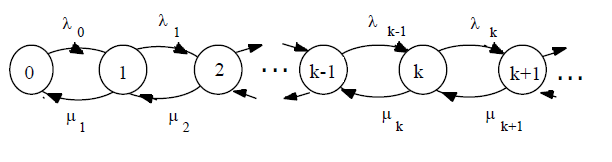
\includegraphics[width=15cm, keepaspectratio]{img/process_nasc_morte.png}
	\caption{Processi di nascita-morte.}\label{fig:nascita_morte}
\end{figure}


Consideriamo un processo di nascita-morte a tempo continuo. In tal caso definiamo la matrice $Q = [q_{ij}]$ delle velocità di transizione fra stati i,$j\in E$, come:
\begin{align}
    & q_{i i+1} = \lambda_i & i \geq 0\\
    &q_{i i+1} = \mu_i & i \geq 0\\
    & q_{00} = -\lambda_0&\\
    & q_{ii} = -(\lambda_i + \mu_i) & i \geq 1\\
    & q_{ij} = 0 & \textrm{per}  |i-j| >1
\end{align}
Il processo è omogeneo perché questi tassi dipendono solo dallo stato e non dal tempo.\\
Il sistema di equazioni $\frac{\mathrm{d \pi (t)} }{\mathrm{d} t} = \pi(t) Q$  relativo alla distribuzione di probabilità di stato $\pi(t)$ al tempo t>0 per un processo di nascita e morte assume la forma seguente:
\begin{align}
    & \frac{\mathrm{d \pi_0 (t)} }{\mathrm{d} t} =  \mu_1 \pi_1(t) -\lambda_0 \pi_0(t) \\
    & \frac{\mathrm{d \pi_k (t)} }{\mathrm{d} t} =  \lambda_{k-1} \pi_{k-1}(t) + \mu_{k+1} \pi_{k+1}(t) - (\lambda_k + \mu_k) \pi_k(t)   & k >0\\
\end{align}

Questo sistema di equazioni descrive il comportamento del processo in funzione del
tempo e può essere risolto assumendo una distribuzione di probabilità di stato iniziale, riguarda la parte dell'analisi transiente.
\\
Se il processo di nascita e morte è irriducibile la probabilità stazionaria di stato $\pi$ si ottiene dalla soluzione del sistema di equazioni di bilanciamento globale che può essere riscritto come:
\begin{align}
    &\mu_1 \pi_1 = \lambda_0 \pi_0\\
    & \lambda_{k-1} \pi_{k-1} + \mu_{k+1} \pi_{k+1} = (\lambda_k + \mu_k)\pi_k & k>0\\
\end{align}
Questo sistema può essere facilmente risolto ad esempio per sostituzione. Infatti dalla
prima equazione si ricava
\[\pi_1 = \pi_0 \dfrac{\lambda_0}{\mu_1}\]
e per sostituzione, dalla seconda equazione
\[\pi_2 = \pi_1 \dfrac{\lambda_1}{\mu_2} = \pi_0 \dfrac{\lambda_1 \lambda_0}{\mu_2 \mu_1}\]
e, per sostituzioni successive, dall’equazione k-sima
\[\pi_k = \pi_{k-1} \dfrac{\lambda_{k-1}}{\mu_{k}} =\pi_0 \prod_{i=0}^{k-1} \dfrac{\lambda_i}{\mu_{i+1}}\]
per k>0.

\paragraph{Condizione di stazionarietà}
Una condizione necessaria e sufficiente perché il processo di nascita e morte sia
ergodico (irriducibile, aperiodico, ricorrente non nullo)  è che esista un $k_0>0$
tale che $\forall k > k_0 $ sia $\lambda_k < \mu_k$ , ovvero $\rho = \dfrac{\lambda}{\mu} < 1 $. Questo vuol dire che se la velocità degli arrivi è maggiore di quella delle partenze allora il sistema è congestionato.

\subsection{Processo di pura nascita}
Considerando il particolare processo di nascita e morte in cui i tassi di morte sono
nulli ($\mu_k=0, k>0$), definiamo un processo di \textbf{pura nascita}. Assumiamo inoltre che il
tasso di nascita sia costante, indipendente dallo stato:$\lambda_k = \lambda, k \geq 0$.

\begin{figure}[H]
	\centering
    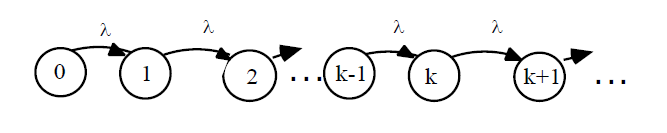
\includegraphics[width=15cm, keepaspectratio]{img/processo_pura_nascita.png}
	\caption{Diagramma di un processo di pura nascita.}\label{fig:diagr_pura_nascita}
\end{figure}

Assumendo la condizione iniziale di sistema vuoto, $\pi_0(0) = 1, \pi_k(0) = 0, \forall k\neq 0$, si ricava facilmente la soluzione transiente:
\begin{align}
    & \pi_k(t)= \dfrac{(\lambda t)^k}{k!} e^{-\lambda t} & k\geq 0, t\geq 0
\end{align}
che riconosciamo, in accordo alla formula \ref{eq:prob_poisson}, come la distribuzione di Poisson di
parametro $\lambda t$, di media e varianza $\lambda tt$.

\subsection{Processo di Poisson}
Indichiamo con N(t), $t\geq0$, il numero di eventi osservati in un intervallo di tempo [0,t], nel caso di un sistema aperto esso rappresenta il numero di arrivi nel suddetto intervallo (\textbf{processo di arrivo}).Inoltre sia $X_i$ la v.c. che indica il tempo che intercorre fra l’arrivo dell’(i-1)-esimo job e l’arrivo dell’i-esimo job al sistema, per i>1, con $X_1$ indichiamo l'arrivo del primo job. Se le v.c. $X_i$, i>0, sono indipendenti ed identicamente distribuite, allora il processo stocastico $\{N(t) | t\geq0\}$ è di rinnovamento. Inoltre se le v.c. $X_i$, i>0, sono i.i.d. con distribuzione esponenziale di parametro $\lambda$ il quale indica il tasso di arrivo, allora il processo stocastico $\{N(t) | t\geq0\}$ è di Poisson. La distribuzione di probabilità di Poisson con parametro $\lambda t$ è data dalla seguente formula:
\[Prob\{N(t) = i\} = e^{-\lambda t} \dfrac{(\lambda t)^i}{i!}\]
\[E[N(t)] = Var[N(t)] = \lambda t\] \label{eq:prob_poisson}
con $i\geq 0$.
Il processo di Poisson può essere definito come il processo stocastico che indica il numero di eventi osservati in un intervallo di tempo [0,t], e che soddisfa le seguenti condizioni:
\begin{itemize}
    \item il numero di eventi in intervalli disgiunti sono stocasticamente indipendenti;
    \item il numero di eventi in un intervallo di tempo dipende solo dalla sua lunghezza e non dall'istante iniziale;
    \item per un valore piccolo di t e per una costante positiva $\lambda$ si ha che:
        \begin{itemize}
             \item Prob \{ un evento in un intervallo di ampiezza t \} = $\lambda t + o(t)$
             \item Prob \{ nessun evento in un intervallo di ampiezza t \} = $o(t)$
             \item Prob \{ più di un evento in un intervallo di ampiezza t \} = $o(t)$ dove $o(t) = \lim_{t \to \infty} [o(t)/t] = 0$.
        \end{itemize}
\end{itemize}
Dalla seconda proprietà deriva che
\[Prob\{ \textrm{k eventi nell'intervallo (s,s+t)}\}= e^{-\lambda t} \dfrac{(\lambda t)^k}{k!}\]
In questo caso se il tempo di interarrivo è esponenziale allora il processo di arrivo è di Poisson e viceversa. Indichiamo con la X la variabile casuale tempo di interarrivo con distribuzione cumulativa $A(t) = Prob\{X \leq t\}$ allora possiamo scrivere che 
\[A(t) = Prob\{N(t) = 0\} = 1 - e^{-\lambda t}, \textrm{ con t>0}\]


\subsubsection{Composizione di processi di Poisson}
La sovrapposizione o composizione di n processi di Poisson indipendenti rispettivamente di parametro $ \lambda_{1}, \lambda_{2} , ..., \lambda_{n}$ è anch’esso un processo di Poisson di parametro $\lambda_{1}+\lambda_{2} +…+\lambda_{n} $.

\subsubsection{Decomposizione di processi di Poisson}
Dato un processo di Poisson $\{N(t) | t\geq 0\}$ di parametro $\lambda$, assumiamo che sia decomposto in n processi, selezionando ogni uscita del processo secondo una distribuzione di probabilità di Bernoulli ad n uscite, con probabilità $p_i, 1\leq i \leq n$. Allora gli n processi di uscita $\{N_i(t)| t\geq 0\} $ sono indipendenti e sono anch'essi processi di Poisson rispettivamente con parametro $\lambda p_i, 1\leq i \leq n$.



    \newpage
    \chapter{Modelli a singola coda}
Un modello a cosa è costituito dalla rappresentazione di un sistema di congestione in cui utenti che provengono da una popolazione si mettono in coda per ottenere il servizio richiesto da un insieme di risorse o serventi. Una coda è una linea di attesa per un servizio. L'insieme formato da cosa e serventi è detto \textbf{centro di servizio}. 

\begin{figure}[H]
	\centering
    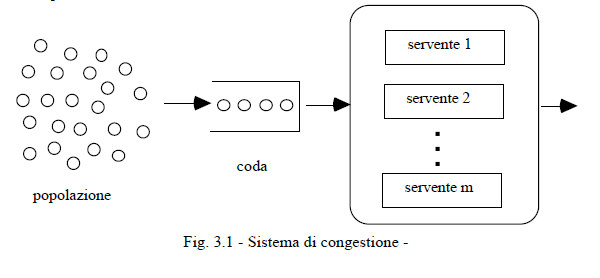
\includegraphics[width=15cm, keepaspectratio]{img/modello_coda.png}
	\caption{Sistema di congestione.}\label{fig:modello_coda}
\end{figure}
Un sistema a coda è costituito da alcune grandezze che sono:
\begin{itemize}
    \item $\Delta$ tempo di interarrivo;
    \item w numero di utenti in cosa e $t_w$ tempi di attesa in coda, tempo che intercorre fra l'arrivo di un utente e l'istante in cui entra in servizio;
    \item s numero di utenti in coda e $t_s$ tempo di servizio, tempo fra inizio e completamento del servizio;
    \item q numero di utenti nel sistema e $t_q$ tempo di risposta, tempo fra arrivo e partenza dal sistema dello stesso utente.
\end{itemize}
Per definizione $q= w+s$ e le variabili di tempi sono legati dalla seguente relazione $t_q = t_w + t_s$.

Fra queste tipicamente alcune sono parametri del sistema, quali $t_s$ e $\Delta$ mentre le altre sono oggetto di analisi e di valutazione.
\paragraph{Processo di arrivo}
Assumiamo che il tempi di interarrivo $ \Delta$ siano variabili casuali statisticamente indipendenti con la stessa distribuzione di probabilità.
\paragraph{Domanda di servizio, tasso di servizio e tempo di servizio}
La quantità di servizio richiesta da un utente ad un centro di servizio è detta
domanda di servizio ed è espressa in unità di tempo. La velocità o tasso di servizio di un servente è una caratteristica del servente, ovvero della risorsa, ed è espressa in unità di servizio per unità di tempo. Il tempo di servizio è la il rapporto fra la domanda di servizio e la velocità di servizio espresso in unità di tempo.
\paragraph{Disciplina di servizio}
Una \textbf{disciplina di servizio} è un algoritmo di ordinamento degli utenti in coda in base al quale viene selezionato l'utente da servire, ovvero l’ordine con cui estrarre gli utenti dalla coda. Alcuni esempi sono FIFO che serve gli utenti in ordine di arrivo  e LIFO che serve gli utenti in ordine inverso al tempo di
arrivo. La disciplina di servizio RAND determina l’utente da estrarre dalla coda e servire
in modo casuale, secondo la distribuzione unforme discreta. Le \textbf{discipline a priorità} determinano l’ordine di servizio degli utenti sulla base di priorità assegnate ad esse. La disciplina round robin è un esempio di disciplina che dipende dalla quantità di servizio già assegnato. Tale algoritmo assegna il servente ciclicamente agli utenti per un intervallo massimo di tempo detto quanto.

\subsection{Notazione di Kendall} Per descrivere e definire i modelli a coda singola Kendall
ha introdotto la seguente notazione:
\[ A/B/c/n/p/Z\]
dove i simboli denotano:
\begin{itemize}
    \item A : distribuzione del tempo di interarrivo;
    \item B : distribuzione del tempo di servizio $t_s$;
    \item c : numero di serventi m;
    \item n : dimensione della coda ovvero la capacità del centro, q;
    \item p : dimensione della popolazione;
    \item  Z : disciplina di servizio.
\end{itemize}
 Tale notazione si semplifica in A/B/c quando coda e popolazione sono illimitate e
la disciplina di servizio è FIFO, ovvero se $n=p=\infty$ e Z=FIFO. D denota la distribuzione deterministica o costante, M la distribuzione esponenziale negativa,$H_h$ l’iperesponenziale ad h stadi,$E_k$ l’Erlangiana a k stadi e G la generale.
Il comportamento del sistema nel tempo può essere analizzato in un tempo finito.
In tal caso si parla di \textbf{analisi transiente}. Quando il sistema raggiunge le condizioni di
equilibrio in un tempo che tende ad infinito, ovvero se il sistema è stabile si effettua
\textbf{l’analisi stazionaria.} Tale analisi porta alla valutazione degli indici di prestazione del sistema di code, in particolare di:
\begin{itemize}
    \item numero di utenti nel sistema q;
    \item numero di utenti in coda w;
    \item tempo di risposta $t_q$;
    \item tempo di attesa $t_w$;
    \item utilizzazione U;
    \item throughput X.
\end{itemize}
Le prime quattro sono variabili casuali di cui si valuta la distribuzione di probabilità,
e/o i momenti. Possiamo scrivere immediatamente le seguenti
relazioni fra i valori medi:

\begin{align}
    & E[q] = E[w] + E[s]\\
    & E[t_q] = E[t_w] + E[t_s]
\end{align}

Una relazione fondamentale nella teoria delle code è rappresentato dal \textbf{teorema di
Little} il quale stabilisce che il numero medio di utenti in un sistema è uguale al
prodotto fra il throughput e il tempo medio di risposta, ovvero:

\begin{align}
   & E[q] = X E[t_q] \\
   & E[w] = X E[t_w]
\end{align}

\subsection{Modelli basilari di code: i sistemi M/M/1 ed M/M/m}
M/M/1 costituisce la base per la definizione di modelli più
complessi a struttura reticolare e per lo sviluppo gerarchico di modelli a diversi livelli
di astrazione. Nella notazione di Kendall il sistema di code M/M/1 denota un sistema aperto
formato da un singolo centro di servizio con:
\begin{itemize}
    \item distribuzione del tempo di interarrivo esponenziale, di parametro $\lambda$,
    \item tempo di servizio degli utenti indipendente e con identica distribuzione
esponenziale di parametro $\mu$,
    \item singolo servente.
\end{itemize}
La disciplina di servizio è FIFO e sia la memoria che la popolazione sono infinite.
\begin{figure}[H]
	\centering
    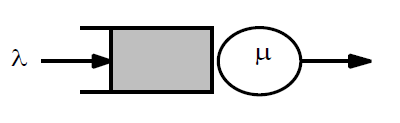
\includegraphics[width=13cm, keepaspectratio]{img/sistema_mm1.png}
	\caption{Sistema M/M/1.}\label{fig:mm1}
\end{figure}

Per le ipotesi di esponenzialità dei tempi di interarrivo e di servizio, gli unici eventi possibili che si osservano in un intervallo di tempo $d_t$ quando nel sistema vi sono k utenti sono i seguenti:
\begin{enumerate}
    \item nessun arrivo e nessun completamento di servizio (permanenza nello stato k);
    \item un arrivo e nessun completamento di servizio (transizione dallo stato k allo stato k+1
con probabilità $\lambda dt$);
    \item nessun arrivo e un completamento di servizio (transizione dallo stato k allo stato k-1
con probabilità $\mu dt$);
    \item uno o più arrivi e uno o più completamenti di servizio (transizione con probabilità
trascurabile rispetto alle altre transizioni per l’ipotesi di esponenzialità).
\end{enumerate}

\subsection{Analisi stazionaria}
Definiamo l’intensità di traffico del sistema come rapporto fra tempo medio di servizio e tempo medio di interarrivo, denotato da $\rho = \lambda / \mu$. La condizione di
stazionarietà del sistema M/M/1 richiede che $\rho <1$, ovvero che il tasso di arrivo al
sistema sia minore del tasso di servizio, $\lambda < \mu$. La distribuzione di probabilità di stato in
equilibrio  si ricava :
\begin{align}
    & \pi_0 = 1- \rho \\
    &\pi_k = \rho^k \pi_0 = \rho (1-\rho) & k>0
\end{align}
la distribuzione di probabilità del numero di utenti nel sistema in condizioni stazionarie è geometrica a ragione $\rho$. \\
Il numero medio di utenti nel sistema, che denotiamo con N=E[q], si può immediatamente ricavare come:
\begin{align}
    N = \frac{\rho }{1-\rho} 
\end{align}
e la varianza del numero di utenti, denotata da Var[q], è
\begin{align}
    Var[q] = \frac{\rho}{(1-\rho)^2}
\end{align}
Per la relazione (5.1) ricaviamo immediatamente il numero medio di utenti in coda,
denotato da W=E[w], poiché $E[s] =\rho$ ed E[q]=N:
\begin{align}
    W = N-\rho = \frac{\rho^2 }{1-\rho}
\end{align}

Il tempo medio di risposta, denotato da R=E[tq], si ricava dal teorema di Little  che per il sistema M/M/1 assume la forma $N= \lambda R$:
\begin{align}
    R = \frac{\frac{1}{\mu}}{1-\rho}
\end{align}

Infine il tempo medio di attesa in coda,$T_w=E[t_w]$ si ottiene o dal teorema di Little come $W = \lambda T_w$ o dalla relazione (3.4) ovvero $R = T_w +T_s$, dove $T_s = \frac{1}{\mu}$ denota il tempo medio di servizio, da cui si ricava
\begin{align}
    T_w = \frac{\frac{\rho}{\mu}}{1-\rho}
\end{align}

L’utilizzazione è esprimibile per il sistema M/M/1 come:
\begin{align}
    U = 1 -\pi_0 = \rho
\end{align}

Dalla distribuzione di probabilità (5.6) possiamo calcolare la probabilità con cui si
osservano almeno k utenti nel sistema in condizioni di equilibrio:
\begin{align}
    & Prob \{ \textrm{numero di utenti nel sistema $\geq$ k}\}= \sum_{i\geq k}^{} \pi_i= (1-\rho) \sum_{i\geq k}^{} \rho_i =\rho^k
\end{align}

\subsection{Sistema M/M/$\infty$ : serventi infiniti}
Un modello M/M/$\infty$ permette di rappresentare un sistema nel quale ad ogni
arrivo vi è sempre un servente libero.In un sistema di questo tipo non si forma quindi
mai coda, poiché ogni utente riceve immediatamente servizio dall’istante in cui arriva
al sistema. Il processo stocastico {q(t) | t>0} associato al sistema $M/M/\infty$ è un processo di
nascita e morte con tassi di nascita $\lambda_k=\lambda, k\geq0, $e con tassi di morte $\mu_k= k \mu, k\geq1$. La condizione di stazionarietà è certamente sempre soddisfatta quindi il
sistema è sempre stabile. esiste la distribuzione stazionaria del numero di utenti nel
sistema, che coincide con il numero di serventi occupati da cui si ricava:
\begin{align}
    & \pi_k = \frac{\rho^k}{k!} e^{-\rho} & k\geq 0
\end{align}
dove $\rho = \lambda/\mu$.
Si ricava immediatamente il numero medio di utenti nel sistema 
\begin{align}
    N = \rho
\end{align}
Dato che nel sistema $M/M/\infty $ gli utenti non sperimentano mai coda, il tempo medio
di risposta coincide con il tempo medio di servizio:
\begin{align}
    R = T_s = \frac{1}{\mu}
\end{align}

\subsection{Sistema M/M/m: serventi multipli}
Il sistema aperto M/M/m è caratterizzato da un processo di arrivo Poissoniano di $\lambda$
parametro, distribuzione del tempo di servizio esponenziale di parametro $\mu$ e un
numero di serventi m>0. Come in M/M/1  il tasso medio di servizio dipende dallo stato k secondo la seguente funzione $\mu(k) = k \mu$ ,$0\leq k\leq m, e \mu(k) = m \mu, k>m$.  Definiamo l’intensità di traffico come $\rho =\lambda/ m\mu$. In questo caso esiste la distribuzione stazionaria del numero di utenti nel sistema :
\begin{align}
    & \pi_k = \frac{(m\rho)^k}{k!}\pi_0 & 0\leq k \leq m \\
    &\pi_k = \frac{m^m \rho^k}{m!}\pi_0 & k>m \\
    &\pi_0 = \left [  \sum_{k=0}^{m-1} \frac{(m\rho)^k}{k!} +  \frac{(m\rho)^m}{m!}\cdot \frac{1}{1-\rho} \right ]^{-1}
\end{align}
Il numero medio di serventi occupati E[s] è dato da
\begin{align}
    & E[s] = \sum_{k=0}^{m-1} k \pi_k + \frac{m\pi_m}{1-\rho} = m\rho = \frac{\lambda}{\mu}
\end{align}
dove $\rho$ rappresenta l’utilizzazione di ogni singolo servente.
Il numero medio di utenti nel sistema è dato da
\begin{align}
    & N = m \rho + \pi_m \frac{\rho}{(1-\rho)^2} \\
    & W = \pi_m \frac{\rho}{(1-\rho)^2}
\end{align}
Il tempo medio di risposta si ottiene applicando il teorema di Little $N=\lambda R$ ottenendo:
\begin{align}
    R = \frac{1}{\mu} + \frac{\pi_m}{(m\mu(1-\rho)^2)}
\end{align}

Similmente, otteniamo il tempo medio di attesa:
\begin{align}
    T_W = \frac{\pi_m}{m\mu ( 1-\rho)^2}
\end{align}
La probabilità che un utente in arrivo trovi tutti i serventi occupati e quindi
sperimenti coda è data dalla formula di Erlang-C:
\begin{align}
    Prob\{\textrm{coda}\} = \sum_{k=m}^{\infty}\pi_k = \pi_0 \frac{(m\rho)^m}{!m} \cdot \frac{1}{1-\rho}
\end{align}
Questa formula, è stata applicata per lo studio di sistemi di traffico telefonico per valutare la probabilità che una chiamata (un utente) trovi tutti i canali di comunicazione (i serventi) occupati.
\\
Vedere esercizio \ref{es:m/m/m}.

\subsection{Sistema M/M/1/K : memoria finita}
Consideriamo il sistema M/M/1 nel quale sono ammessi al più K utenti. Il processo di arrivo è Poissoniano di parametro $\lambda$, ma un utente che arrivando trova il sistema completo, cioè con K utenti già presenti, non viene accettato e viene perso. Il processo stocastico ${q(t) | t>0}$ associato al sistema M/M/1/k è un processo di nascita e morte con spazio degli stati finito $E=\{0,1,\cdots, K\}$ e tassi di nascita $\lambda_k=\lambda$,$ 0 \leq k<K$, e tassi di morte $\mu_k= \mu$, $1\leq k<K-1$ e $\lambda_k=0$ e $\mu_k= 0$ altrove. La condizione di stazionarietà è certamente verificata, poiché il processo è finito e irriducibile e quindi ergodico. La distribuzione stazionaria del numero di utenti nel sistema
definita dalle formule:
\begin{align}
    & \pi_k = \frac{1-\rho}{1 -\rho^{K+1}} \rho & 0\leq k \leq K \\
    & \pi_k = 0 & k>K
\end{align}
Nel caso particolare di K=1 lo spazio è formato da due soli stati e si ricava
\begin{align}
    & \pi_0 = \frac{\mu}{\lambda +\mu}\\
    & \pi_1 = \frac{\lambda}{\lambda + \mu}
\end{align}

\subsection{Sistema M/M/1//M: popolazione finita}
Consideriamo il sistema M/M/1 assumendo che gli utenti provengano da una popolazione finita, di dimensione M>0.
    \newpage
    \chapter{Analisi di risultati e convalida in esperimenti di simulazione}

\section{Stima dei parametri di una distribuzione}
\subsection{Stima della media}
Sia data una popolazione la cui distribuzione f(x) è stazionaria (cioè costante nel tempo), con media $E(x) = \eta $ e varianza $\sigma^2(x)= \sigma^2$. Facciamo n osservazioni indipendenti $x_1,x_2,x_3,...,x_n$ che chiamiamo \textbf{campione}. Le media del campione è 
\[ \bar{x} = \dfrac{1}{n}\sum_{i=1}^{n} x_i\]
è detta \textbf{media campionaria}.
Allora 
\[E(\bar{x}) = \eta\]
\[\sigma^2 = \dfrac{\sigma^2}{n}\]

La costante 1-$\alpha$, usualmente espressa in percentuale, è detta di livello di confidenza per la stima $\eta$ e l'intervallo 
\[ \bar{x} \pm \dfrac{\sigma}{\sqrt{n}} u_{\dfrac{\alpha}{2}}\]
è detto \textbf{intervallo di confidenza}. Ad esempio con un livello di confidenza pari a 95\% allora 
\[1-\alpha = 0,95, \alpha = 0,05, \dfrac{\alpha}{2}= 0,025, 1- \dfrac{\alpha}{2}= 0.975\]
Dalla tavola di distribuzione si ricava che per $F(u_{\dfrac{\alpha}{2}})= 0.975, u_{\dfrac{\alpha}{2}}= 1.96$ .
Ciò vuol dire che su 100 campioni, ciascuno di n osservazioni, in 95 di essi l'intervallo $\bar{x} \pm 1,96 \dfrac{\sigma}{\sqrt{n}}$ conterrà il valore $\eta$.
Nella pratica la varianza $\sigma^2$ della popolazione non è nota. In tal caso, la si sostituisce con la varianza del campione, definita come:
\[ s^2 = \dfrac{1}{n-1} \sum_{i=1}^{n}(x_i- \bar{x})^2\]
e la variabile standard 
\[ t = \dfrac{\bar{x}-\eta}{s/\sqrt{n}}\]

\subsection{Stima della varianza}
Il metodo indiretto  per la stima di $\sigma^2(x)$ è quello che usa la relazione $\sigma^2(x)= E(x^2) -E^2(x)$ e passa dalla stima di E(x) a quella di $\sigma^2(x)$. Se ho la media la calcolo al quadrato e ho il secondo termine dall'equazione $\sigma^2(x)= E(x^2) -E^2(x)$ , poi avendo tutti i campioni li elevo al quadrato e calcolo la media di questi, in questo modo si trova la varianza.

\section{Stima della distribuzione}
\subsection{Metodo del coefficiente di variazione}
Si definisce coefficiente di variazione di una distribuzione teorica il rapporto tra la deviazione standard e la media:
\[ \nu  = \dfrac{\sigma}{\eta}\]
Se $\nu=0$ allora la distribuzione è una costante(deterministica).
Esso definisce una misura di come i valori della variabile sono dispersi intorno alla media. Per le distribuzioni viste sinora abbiamo:
\begin{align*}
    & \nu(esponenziale) = \dfrac{1/\lambda}{1/\lambda} =1\\
    & \nu(Erlang-k) = \dfrac{1/(\sqrt{k}\lambda)}{1/\lambda} = \dfrac{1}{\sqrt{k}} & k=1,2,....\\
\end{align*}
\subsection{Metodo del goodness of fit}
Il numero delle osservazioni deve essere maggiore di 30, sennò si usa il metodo del Kolmogorov-Smirnov. Supponiamo di aver fatto un campione di n osservazioni a partire da una popolazione continua reale e averne tracciato il relativo istogramma. Il procedimento che andremo a effettuare con una distribuzione normale può essere applicato ad altri tipi di distribuzioni continue di cui sia nota l'espressione della funzione cumulativa.

\subsubsection{Esempio dal Capitolo 5}
I dati di questo esempio sono i seguenti.
\begin{figure}[H]
	\centering
    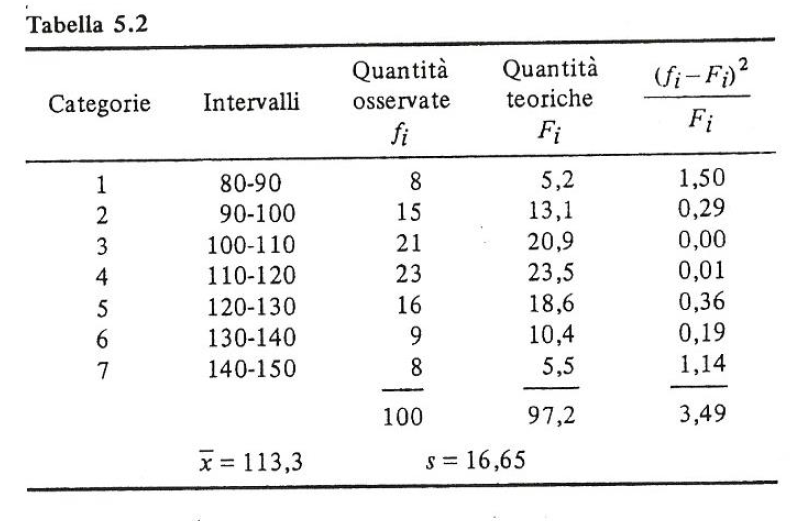
\includegraphics[width=15cm, keepaspectratio]{img/esercizio_good_fit.png}
	\caption{Tabella esempio stima distribuzione.}\label{fig:good_fit}
\end{figure}
Innanzitutto bisogna controllare il numero di osservazioni se è maggiore di $n>30$ allora possiamo applicare il metodo, inoltre suddividendo i campioni in categorie dobbiamo controllare che ci siano almeno 5 $f_i > 5$osservazioni per categoria.\\
Calcoliamo la media del campione $\bar{x}$
\[ \bar{x} = \dfrac{1}{n} \sum_{i=1}^{n} x_i = \dfrac{85\cdot8 + 95 \cdot 15 + 105 \cdot21 + 115 \cdot 23 +125 \cdot 16 + 135 \cdot9 + 145 \cdot8 }{100} = 113,3\]
Calcoliamo la deviazione standard dalla varianza $s$

\begin{equation*}
     s= \sqrt{s^2} = \sqrt{\begin{multlined}[b] 
     \dfrac{1}{n-1} \cdot [ (85\cdot8)^2 + (95 \cdot 15)^2 +\\
     (105 \cdot21)^2 +( 115 \cdot 23)^2 +(125 \cdot 16)^2 +\\
     (135 \cdot9)^2 + (145 \cdot8)^2 = 16,65]
     \end{multlined}}
\end{equation*}
    
Poi facciamo il rapporto fra le due ovvero
\[\nu = \frac{16}{113}\]
Essendo che è una normale il rapporto è un numero lontano da 1, al contrario di una esponenziale negativa.
    \newpage
    
\chapter{Esercizi}

\section{Esercizio su M/M/m} \label{es:m/m/m}
La clinica oculistica dell’Ospedale offre ogni mercoledì pomeriggio dei test gratuiti della vista.
Ci sono 3 oculisti in contemporanea. Un test impiega, in media, 20 minuti e il tempo reale è stato
riscontrato essere approssimativamente distribuito in modo esponenziale intorno a questa media.
I clienti arrivano in accordo ad un processo di Poisson con un tasso medio di 6 all’ora e i pazienti
sono serviti seguendo una politica FIFO.\\

\noindent I dirigenti dell’Ospedale sono interessati a conoscere:
\begin{enumerate}
    \item Quale è il numero medio di persone in attesa?
    \item Quale è il tempo medio speso da un paziente nella clinica?
    \item Quale è la percentuale media del tempo in cui i dottori non lavorano?
    \item Quale è la frazione di tempo nella quale un cliente che arriva trova almeno 1 dottore libero.
\end{enumerate}

\subsection{Soluzione}
Troviamo alcuni parametri, m=3 $\mu= \frac{1}{20}/min = \frac{20}{60} = \frac{1}{3}/ora$ questo vuol dire che in un ora vengono effettuate 3 visite, $\lambda = 6/ora$ quindi
\[\rho = \frac{\lambda}{\mu m} = \frac{6}{3 \cdot 3} = \frac{2}{3} < 1 \]

\begin{enumerate}
    \item  Il numero medio di persone in attesa è
            \begin{align*}
                 & W = \pi_m \frac{\rho}{(1-\rho)^2} = \frac{4}{27} \cdot \frac{2/3}{(1-2/3)^2} = \frac{8}{9}\\
                 & \pi_0 = \left [  \sum_{k=0}^{m-1} \frac{(m\rho)^k}{k!} +  \frac{(m\rho)^m}{m!}\cdot \frac{1}{1-\rho} \right ]^{-1} = \left [  \sum_{k=0}^{2} \frac{(3 \cdot 2/3)^k}{k!} +  \frac{(3 \cdot 2/3)^3}{3!}\cdot \frac{1}{1-2/3} \right ]^{-1} = \\
                 & \left [ \frac{2^0}{0!}+ \frac{2^1}{1!} + \frac{2^2}{2!} + 4 \right]^{-1} = [9]^{-1} = \frac{1}{9}\\
                 & \pi_k = \frac{(3\cdot 2/3)^3}{3!} \frac{1}{9} = \frac{8}{54} = \frac{4}{27}
            \end{align*}
    
    \item Il tempo medio speso da un paziente nella clinica è:
            \begin{align*}
                   & R = \frac{1}{\mu} + \frac{\pi_m}{(m\mu(1-\rho)^2)} = \frac{1}{\frac{1}{20}} + \frac{}{}\pi_m
            \end{align*}
\end{enumerate}


    \newpage
    % ...
    \bibliographystyle{plainnat}
    % Opzionale
    \newpage
    % \bibliography{bibliografia}
	

    
\end{document}
